\documentclass[oneside,14pt]{extarticle}
\usepackage{cmap}
\usepackage[utf8]{inputenc}
\usepackage[english,ukrainian]{babel}
\usepackage{graphicx}
\usepackage{geometry}
\usepackage{listings}
\usepackage{float}
\usepackage{amsmath}
\usepackage{subfig}
\geometry{
	a4paper,
	left=20mm,
	right=20mm,
	top=15mm,
	bottom=15mm,
}
\lstset{
	language=c,
	tabsize=4,
	keepspaces,
	showstringspaces=false,
	frame=single,
	breaklines,
	language=C,
}
\graphicspath{ {./pictures} }
\setlength{\parindent}{4em}

\newcommand\subject{Основи програмування вбудованих систем}
\newcommand\lecturer{доцентка кафедри ПЗ\\Марусенкова Т.А.}
\newcommand\teacher{доцент кафедри ПЗ\\Крук О.Г.}
\newcommand\mygroup{ПЗ-32}
\newcommand\lab{3}
\newcommand\theme{Робота з потоками у CMSIS-RTOS}
\newcommand\purpose{Навчитися управляти потоками у операційній системі CMSIS-RTOS у середовищі Keil uVision}

\begin{document}
\begin{normalsize}
	\begin{titlepage}
		\thispagestyle{empty}
		\begin{center}
			\textbf{МІНІСТЕРСТВО ОСВІТИ І НАУКИ УКРАЇНИ\\
				НАЦІОНАЛЬНИЙ УНІВЕРСИТЕТ "ЛЬВІВСЬКА ПОЛІТЕХНІКА"}
		\end{center}
		\begin{flushright}
			\textbf{ІКНІ}\\
			Кафедра \textbf{ПЗ}
		\end{flushright}
		\vspace{80pt}
		\begin{center}
			\textbf{ЗВІТ}\\
			\vspace{10pt}
			до лабораторної роботи № \lab\\
			\textbf{на тему}: <<\textit{\theme}>>\\
			\textbf{з дисципліни}: <<\subject>>
		\end{center}
		\vspace{80pt}
		\begin{flushright}
			
			\textbf{Лекторка}:\\
			\lecturer\\
			\vspace{28pt}
			\textbf{Виконав}:\\
			
			студент групи \mygroup\\
			Коваленко Д.М.\\
			\vspace{28pt}
			\textbf{Прийняв}:\\
			
			\teacher\\
			
			\vspace{28pt}
			«\rule{1cm}{0.15mm}» \rule{1.5cm}{0.15mm} 2024 р.\\
			$\sum$ = \rule{1cm}{0.15mm}……………\\
			
		\end{flushright}
		\vspace{\fill}
		\begin{center}
			\textbf{Львів — 2024}
		\end{center}
	\end{titlepage}
		
	\begin{description}
		\item[Тема.] \theme.
		\item[Мета.] \purpose.
	\end{description}

	\section*{Індивідуальне завдання}
	6. Створити 4 потоки, які засвічують по одному світлодіоду, вимикаючи інші. При цьому перший потік має виконуватися у 2 рази частіше, ніж другий, другий – у два рази частіше, ніж третій і т.д.

	\section*{Теоретичні відомості}
	6. Чи можна потоку змінити пріоритет у ході виконання програми? Якщо так, то яким чином?
	
	Для зміни пріоритету потоку в CMSIS-RTOS, використовується функція osThreadSetPriority().
	
	\begin{lstlisting}
osStatus osThreadSetPriority(osThreadId thread_id, osPriority priority);	\end{lstlisting}
	
	\section*{Хід роботи}
	\begin{figure}[H]
		\centering
		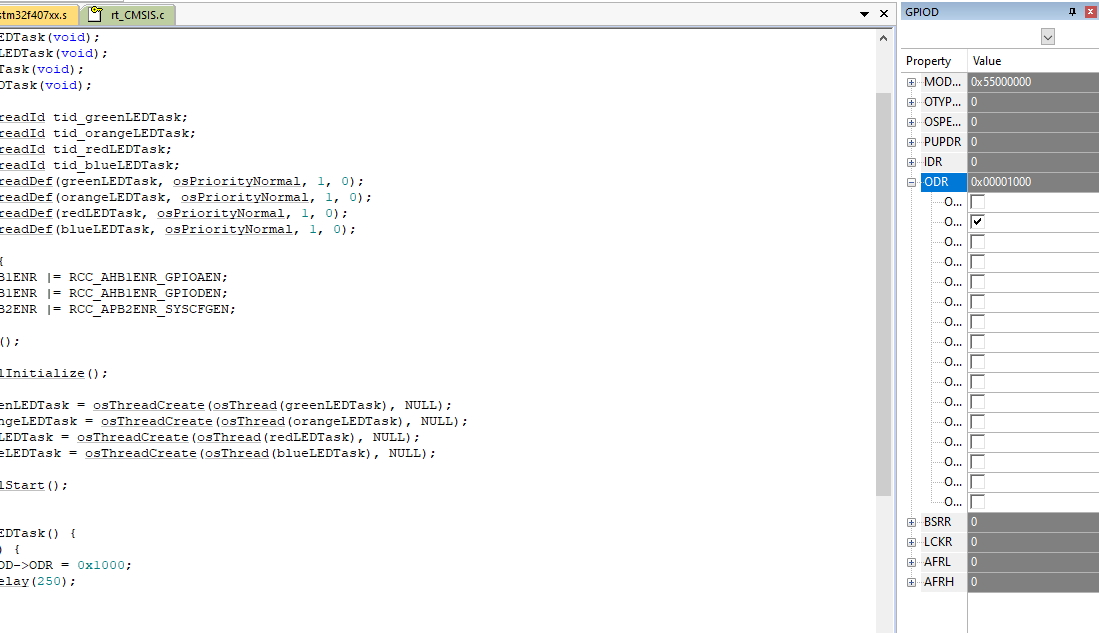
\includegraphics[scale=0.45]{1}
		\caption{Виконання програми.}
	\end{figure}

	\begin{figure}[H]
		\centering
		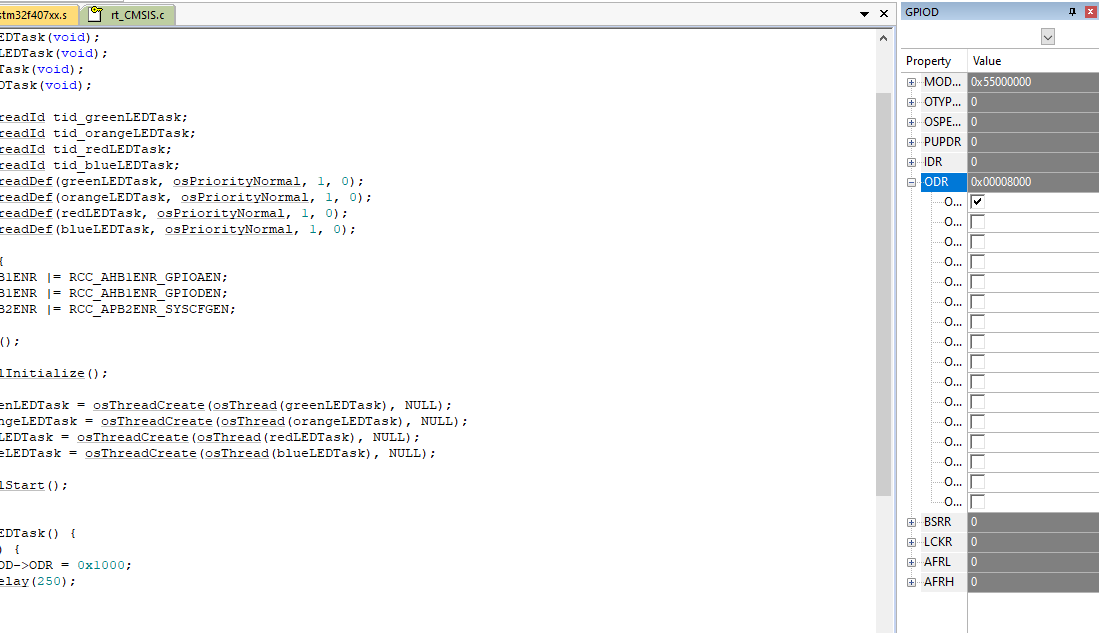
\includegraphics[scale=0.45]{2}
		\caption{Виконання програми.}
	\end{figure}
	
	\begin{figure}[H]
		\centering
		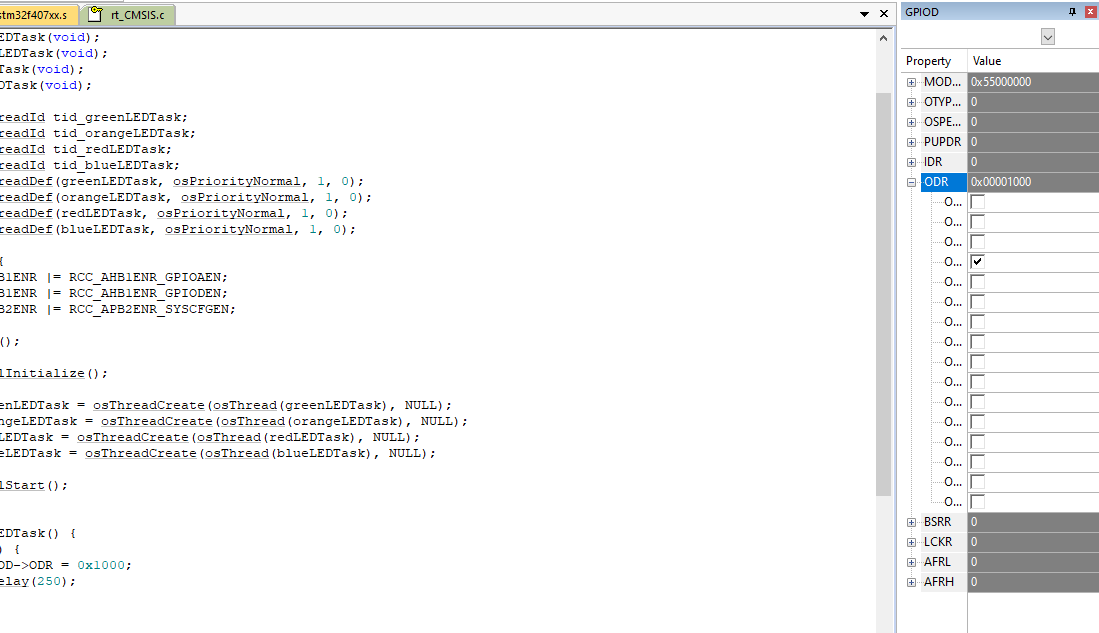
\includegraphics[scale=0.45]{3}
		\caption{Виконання програми.}
	\end{figure}
	
	\subsection*{Код програми}
	Файл \textit{main.c}:
	{\small
		\begin{lstlisting}
#include <stm32f4xx.h>
#include <cmsis_os.h>

void LEDInit(void);

void greenLEDTask(void);
void orangeLEDTask(void);
void redLEDTask(void);
void blueLEDTask(void);

static osThreadId tid_greenLEDTask;
static osThreadId tid_orangeLEDTask;
static osThreadId tid_redLEDTask;
static osThreadId tid_blueLEDTask;
static osThreadDef(greenLEDTask, osPriorityNormal, 1, 0);
static osThreadDef(orangeLEDTask, osPriorityNormal, 1, 0);
static osThreadDef(redLEDTask, osPriorityNormal, 1, 0);
static osThreadDef(blueLEDTask, osPriorityNormal, 1, 0);

int main() {
	RCC->AHB1ENR |= RCC_AHB1ENR_GPIOAEN;
	RCC->AHB1ENR |= RCC_AHB1ENR_GPIODEN;
	RCC->APB2ENR |= RCC_APB2ENR_SYSCFGEN;
	
	LEDInit();
	
	osKernelInitialize();
	
	tid_greenLEDTask = osThreadCreate(osThread(greenLEDTask), NULL);
	tid_orangeLEDTask = osThreadCreate(osThread(orangeLEDTask), NULL);
	tid_redLEDTask = osThreadCreate(osThread(redLEDTask), NULL);
	tid_blueLEDTask = osThreadCreate(osThread(blueLEDTask), NULL);
	
	osKernelStart();
}

void greenLEDTask() {
	while(1) {
		GPIOD->ODR = 0x1000;
		osDelay(250);
	}
}

void orangeLEDTask() {
	while(1) {
		GPIOD->ODR = 0x2000;
		osDelay(500);
	}
}

void redLEDTask() {
	while(1) {
		GPIOD->ODR = 0x4000;
		osDelay(1000);
	}
}

void blueLEDTask() {
	while(1) {
		GPIOD->ODR = 0x8000;
		osDelay(2000);
	}
}

void LEDInit() {
	GPIOD->MODER = 0x55000000;
	GPIOD->OTYPER = 0;
	GPIOD->OSPEEDR = 0;
}
		\end{lstlisting}
	}
	
	\section*{Висновки}
	Під час виконання лабораторної роботи я навчився управляти потоками у операційній системі CMSIS-RTOS у середовищі Keil uVision.
	    
\end{normalsize}
\end{document}
